\documentclass{beamer}
\usepackage{amsmath}
\usepackage{mathtools}
\usepackage[outline]{contour}

\mode<presentation>
{
  \useoutertheme{default}
}

\beamertemplatenavigationsymbolsempty
\setbeamertemplate{frametitle}[default][center]
%\setbeamercolor{frametitle}{fg=white}
%\setbeamercolor{background canvas}{bg=black}
%\setbeamercolor{normal text}{fg=white}
%\usepackage[dvipsnames]{xcolor}
\definecolor{cyan}{rgb}{0,1,1}
\definecolor{yellow}{rgb}{1,1,0}
\definecolor{magenta}{rgb}{1,0,1}

\title{Evolution on graphs and the transition to cancer}
\author{Chay Paterson}
\institute{University of Manchester}
\date{\today}

\begin{document}

\frame{\titlepage}

% Intro: Two slides about differential equations
\begin{frame}
    \frametitle{Introduction}
    \framesubtitle{Differential equations}

    \begin{columns}
        \begin{column}{0.5\textwidth}
        \includegraphics[width=\textwidth]{figures/PIA22946-Jupiter-RedSpot-JunoSpacecraft-20190212.jpg}
        \end{column}
        \begin{column}{0.5\textwidth}
        \includegraphics[width=\textwidth]{figures/Cloud_vortices_off_Cheju_Do_cropped.jpg}
        \end{column}
    \end{columns}
    \begin{center}
    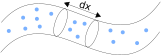
\includegraphics[width=0.5\textwidth]{figures/air}
    \end{center}
\end{frame}

\begin{frame}
    \frametitle{Introduction}
    \framesubtitle{Driver mutations}

    \begin{columns}
        \begin{column}{0.5\textwidth}
        \includegraphics[width=\textwidth]{figures/tumour2.jpg}
        \end{column}
        \begin{column}{0.5\textwidth}
        \includegraphics[width=\textwidth]{figures/covid.png}
        \end{column}
    \end{columns}
    \begin{center}
    \includegraphics[width=0.5\textwidth]{figures/dna.png}
    \end{center}
\end{frame}

\begin{frame}
    \frametitle{Multi-stage models}
    \framesubtitle{P. Armitage and R. Doll\footnotemark[12]}

    \begin{columns}
        \begin{column}{0.5\textwidth}
        \includegraphics[width=\textwidth]{figures/LSHTM-small.jpg}
        \end{column}
        \begin{column}{0.5\textwidth}
        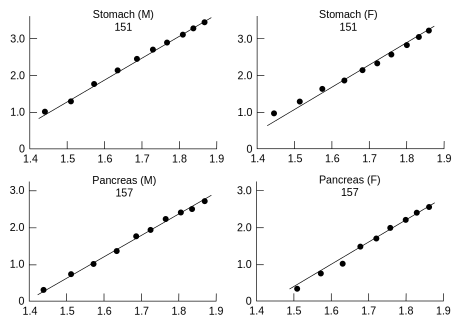
\includegraphics[width=\textwidth]{figures/PArmitageRDoll_1954_6602297.pdf}
        \end{column}
    \end{columns}


\footnotetext[1]{P. Armitage and R. Doll, British Journal of Cancer 1954; 8: 1–12}
\footnotetext[2]{P. Armitage and R. Doll, British Journal of Cancer 1957; 11(2): 161-169}
\end{frame}

\begin{frame}
    \frametitle{Multi-stage models}
    \framesubtitle{A.G. Knudson\footnotemark[12]}

    \begin{columns}
        \begin{column}{0.5\textwidth}
            \includegraphics[width=0.90\textwidth]{figures/Rb_whiteeye.PNG}
            \;
            \includegraphics[width=0.90\textwidth]{figures/retinoblastoma.jpg}
        \end{column}
        \begin{column}{0.5\textwidth}
            \includegraphics[width=0.90\textwidth]{figures/Screenshot_2022-10-31_11-57-01.png}
        \end{column}
    \end{columns}

\footnotetext[1]{AG. Knudson, PNAS 68.4 (1971): 820-823.}
\footnotetext[2]{F. Michor, Y. Iwasa and MA. Nowak, Nature Reviews Cancer 2004; 4: 197-205 doi:10.1038/nrc1295}
\end{frame}

\begin{frame}
    \frametitle{Graphs}

    \begin{columns}
        \begin{column}{0.6\textwidth}
        This network...
        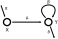
\includegraphics[width=\textwidth]{figures/diagram1}
        \end{column}
        \begin{column}{0.4\textwidth}
        corresponds to this stochastic process:...
        \begin{align}
            \emptyset \rightarrow X, &\qquad \mathrm{rate\;}\alpha
            \nonumber \\
            % NB
            X \rightarrow X + Y, &\qquad\mathrm{rate\;}\mu X
            \nonumber \\
            Y \rightarrow Y + Y, &\qquad\mathrm{rate\;} \beta Y
            \nonumber \\
            Y \rightarrow \emptyset, &\qquad\mathrm{rate\;} \delta Y
            \nonumber
        \end{align}
        \end{column}
    \end{columns}

%    and approximately this linear system...

%    \begin{equation*}
%        \frac{d}{dt} 
%        \begin{pmatrix}
%            E[X] \\
%            E[Y] \\
%        \end{pmatrix}
%        = 
%        \begin{bmatrix}
%            0 & 0 \\
%            \mu & \beta - \delta \\
%        \end{bmatrix}
%        \cdot
%        \begin{pmatrix}
%            E[X] \\
%            E[Y] \\
%        \end{pmatrix}
%        +
%        \begin{pmatrix}
%            \alpha \\
%            0 \\
%        \end{pmatrix}
%    \end{equation*}

\footnotetext[1]{C. Paterson, I. Bozic, H. Clevers, PNAS 2020; 117(34): 20681-20688}
\end{frame}

\begin{frame}
    \frametitle{How do these studies work?}

    What are the relevant observables in this type of longitudinal study \& data
    analysis? 

    Track a cohort that initially contains $N$ patients in the study:

    \begin{itemize}
        \item Age-specific incidence $I(a)$: rate at which new cases are
        recorded in the cohort with ages between $a$ and $a + da$
        \item Survival function $S(a)$: probability to survive to age $a$
        without being diagnosed.
    \end{itemize}

    \begin{equation}
        I(a) = -N \frac{dS}{da} = -N\; S(a) \frac{d \ln S}{da}
    \end{equation}
\end{frame}

\begin{frame}
    \frametitle{So what?}

    \includegraphics[width=1.00\textwidth]{figures/diagram3}

    \begin{itemize}
        \item The survival curve S(a) determines the incidence curve $I(a)$ 
        \item The model determines the survival curve: the probability not to
        end up at one of the end nodes of the graph. We want to know what model+parameters best agree with
        data from studies.
        \item To fit (or ``train'') the model to longitudinal data, we need to compute $S(a)$!
    \end{itemize}

    \;

    This is the central mathematical problem in cancer epidemiology. \emph{How do we compute $S$?}
\end{frame}

\begin{frame}
    \frametitle{Multi-stage clonal expansion models}
    \framesubtitle{2-3 rate limiting steps\footnotemark[123]}
    % TODO present both models
    % ie include Armitage Doll 1957 model, cite Jo Ivasa
    Problem: how to compute $S(t)$ for a given model?

    \begin{columns}
        \begin{column}{0.5\textwidth}
        \begin{center}
        % multi-stage clonal expansion
        \end{center}
        Different methods:
        Fast:
        \begin{itemize}
            \item Armitage + Doll's approximation\footnotemark[1]
            \item Moolgavkar + Venzon's quadrature\footnotemark[2]
        \end{itemize}
        Very slow:
        \begin{itemize}
            \item Gillespie algorithm + sampling \footnotemark[3]
        \end{itemize}
        \end{column}
        \begin{column}{0.5\textwidth}
        \begin{center}
            \includegraphics[width=1.00\textwidth]{figures/diagram3}
            $\downarrow?$
            \includegraphics[width=0.75\textwidth]{figures/ArmitageDoll1957_4A.png}
        \end{center}
        \end{column}
    \end{columns}

    % TODO add figure from Armitage Doll 1957 etc.
\footnotetext[1]{P. Armitage and R. Doll, British Journal of Cancer 1957; 11(2): 161-169}
\footnotetext[2]{S. Moolgavkar and G. Luebeck, JNCI 1992; 84(8): 610-618}
\footnotetext[3]{C. Paterson, I. Bozic, H. Clevers, PNAS 2020; 117(34): 20681-20688 (supp. material)}
\end{frame}


\begin{frame}
    \frametitle{Armitage and Doll's approximation}

    \begin{columns}
        \begin{column}{0.5\textwidth}
            \includegraphics[width=1.00\textwidth]{figures/diagram3}
            \includegraphics[width=0.75\textwidth]{figures/ArmitageDoll1957_4A.png}
        \end{column}
        \begin{column}{0.5\textwidth}
        \begin{itemize}
            \item Assume all the probabilities are small: $1-S \ll 1$
            \item Then the relevant probability $S(a)$ is expressible in terms
            of expected values/population means, which implies
        \end{itemize}
        \begin{equation}
            S(a) \propto a^k (e^{s a} - 1)
        \end{equation}
        with constants $k$ and $s$.
        \begin{itemize}
            \item Don't use correlations, variances, or higher moments in stem
            cell populations -- just ignore these.
        \end{itemize}
        \end{column}
    \end{columns}
\end{frame}

\begin{frame}
    \frametitle{Models on graphs}
    \begin{columns}
        \begin{column}{0.5\textwidth}
        \begin{enumerate}
            \item Most methods for computing $S(a)$ do not consider graphs with
            multiple end nodes
            \item To study \textbf{specific genes} and mechanisms of interest
            (SNVs, LOH, CNA, etc.), we need to evaluate $S(a)$ for a model
            defined on a graph (right)
            \item What methods do we actually have?
        \end{enumerate}
        \end{column}
        \begin{column}{0.5\textwidth}
        \begin{center}
            \small{example model}
        \end{center}
            \includegraphics[width=\textwidth]{figures/diagram4}
        \end{column}
    \end{columns}

    \;

    \begin{center}
        This gets us the incidence of \emph{specific karyotypes}
    \end{center}
\end{frame}


\begin{frame}
    \frametitle{Colorectal adenocarcinoma model}
    \begin{columns}
        \begin{column}{0.5\textwidth}
        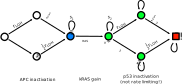
\includegraphics[width=1.0\textwidth]{figures/diagram7}
        \begin{itemize}
            \item Can use A-D type approximation, or stochastic simulations
            %\item Conditional path probabilities $P(X_i)$ encode fitnesses
        \end{itemize}
        but:
        \begin{itemize}
            \item Mean-field breaks down at old ages / large probabilities
            \item Stochastic simulations are \emph{extremely slow}
        \end{itemize}
        \end{column}
        \begin{column}{0.5\textwidth}
        % graph from our PNAS paper
        \includegraphics[width=\textwidth]{figures/F2.large.jpg}
        \end{column}
    \end{columns}

\footnotetext[1]{C. Paterson, I. Bozic, H. Clevers, PNAS 2020; 117(34): 20681-20688}
\end{frame}

\begin{frame}
    \frametitle{Alternative approach: Kolmogorov forward equations}
    Define a more general generating function $\Psi$:

    \begin{equation}
        \Psi(t, \vec{q}) = \mathbb{E}[\left[\prod_j q_j^{N_j}\right]
    \end{equation}

    and derive Kolmogorov forward equations instead. Then we can numerically
    integrate these, and get survival curves $S_i(a)$ for different types of
    cancer $i$. E.G. tumours with clonal LOH, or no clonal LOH.

    \begin{equation}
        S_i = \Psi(t, q_j =1, \dots, q_i = 0)
    \end{equation}
    People knew about this approach for a long time (since 1970s) but it was never
    considered as useful as backward equations.

\footnotetext[1]{SH Moolgavkar and DJ Venzon, Math. biosc. 1979; 47(1): 55-77}
\footnotetext[2]{DW Quinn, Risk Analysis 1989; 9(3): 407-13}
\end{frame}

\begin{frame}
    \frametitle{Kolmogorov forward equations as wave equations}

\begin{center}
        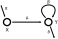
\includegraphics[width=0.4\textwidth]{figures/diagram1}
\end{center}

    Briefly: the Kolmogorov forward equations in $P(N_0, \dots)$
\begin{align}
    \frac{d P(N_0, N_1, \dots)}{dt} &= \sum_{vertices} \alpha (N_j - 1)
    P(\dots, N_j - 1, \dots) \nonumber \\
    &\; - \alpha N_j P(\dots, N_j, \dots) \nonumber \\
    &\; + \beta \cdots + \mu \cdots + \delta \cdots \nonumber
\end{align}

get transformed...

\end{frame}

\begin{frame}
    \frametitle{Kolmogorov forward equations as wave equations}
    They transform with $P \rightarrow \Psi$:
    \begin{equation}
        \frac{\partial \Psi}{\partial t} = \sum_{vertices} \alpha (q_j - 1) q_j
        \frac{\partial \Psi}{\partial q_j} + \dots = \mathcal{H}\Psi
    \end{equation}
    where $\mathcal{H}$ is a hyperbolic differential operator.

    Because this is a hyperbolic wave equation, we can solve for future values
    of $\Psi$ if we have initial values, by evolving them along
    \emph{characteristics}.

\footnotetext[1]{SH Moolgavkar and DJ Venzon, Math. biosc. 1979; 47(1): 55-77}
\end{frame}

\begin{frame}
    \frametitle{Kolmogorov forward equations}

    \begin{columns}
        \begin{column}{0.5\textwidth}
    Using the big generating function $\Psi$, find the corresponding wave
    equation:

    \begin{equation}
        \frac{d \Psi}{ dt} = \mathcal{H} \Psi
    \end{equation}

    This can be solved using the method of characteristics, so we can instead
    integrate

    \begin{equation}
        \frac{d \vec{\gamma}}{ dt} = \vec{X}
    \end{equation}
    numerically, using an appropriate time stepper.


        \end{column}
        \begin{column}{0.5\textwidth}
            \includegraphics[width=\textwidth]{figures/flowcube1}

            \;

            The vector field $\vec{X}$ and a characteristic $\vec{\gamma}$
        \end{column}
    \end{columns}
\footnotetext[1]{SH Moolgavkar and DJ Venzon, Math. biosc. 1979; 47(1): 55-77}
\end{frame}

\begin{frame}
    \frametitle{Random sampling}
    \framesubtitle{Error analysis}

    To compare methods, ask under what conditions the errors are
    similar. Stochastic algorithms have 

    \begin{equation}
        \epsilon \sim N^{-1/2}
    \end{equation}
    and will thus need
    
    \begin{equation}
        N \sim \mathcal{O}(\epsilon^{-2})
    \end{equation}
    runs, so overall runtime $T \propto N$.

\end{frame}

\begin{frame}
    \frametitle{Method of characteristics}
    \framesubtitle{Error analysis}

    Why wasn't this method ever used? Wave equation+characteristic methods were
    studied before, but used Euler integration, which has error
    \begin{equation}
        \epsilon \sim \Delta t
    \end{equation}
    and required two passes, so it ran in
    \begin{equation}
        T \sim \Delta t^{-2} \sim \mathcal{O}(\epsilon^{-2})
    \end{equation}
    this is asymptotically just as bad as random sampling! 
\footnotetext[1]{SH Moolgavkar and DJ Venzon, Math. biosc. 1979; 47(1): 55-77}
\footnotetext[2]{DW Quinn, Risk Analysis 1989; 9(3): 407-13}
\end{frame}

\begin{frame}
    \frametitle{Fast forward method}
    \framesubtitle{Error analysis}
    But what happens if we only need one pass, and replace Euler integration with a Runge-Kutta scheme?

    \begin{equation}
        \epsilon \sim \Delta t^2
    \end{equation}
    and runs in 
    \begin{equation}
        T \sim \Delta t^{-1} \sim \mathcal{O}(\epsilon^{-1/2})
    \end{equation}
    so new runtime $\sim \mathcal{O}\left(\right.$ old runtime
    $\left.^{1/4}\right)$.

    \;

    Amazing!
\end{frame}

\begin{frame}
    \frametitle{Fast forward method}

    \begin{center}
    \includegraphics[height=0.8\textheight]{figures/SCurveComparison.pdf}
    \end{center}

    Random sampling vs fast forward method:

    Monte Carlo: $\approx 5000$s
    Fast forward: 4ms
\end{frame}

\begin{frame}
    \frametitle{Fast forward method}
    \framesubtitle{Error analysis}
    \begin{center}
        \includegraphics[height=0.9\textheight]{figures/Global_error_ffwdmethod_max}
    \end{center}
\end{frame}

\begin{frame}
    \frametitle{How do they compare?}
    \begin{center}
        \includegraphics[height=0.9\textheight]{figures/Error_vs_runtime}
    \end{center}
\end{frame}

\begin{frame}
    \frametitle{Fast forward method}
    Efficiently computing $S_k(a)$ means we can evaluate likelihood functions
    directly, just sampling them.....

    \begin{columns}
        \begin{column}{0.5\textwidth}
        \includegraphics[width=\textwidth]{figures/raster.png}
        \end{column}
        \begin{column}{0.5\textwidth}
        \includegraphics[width=\textwidth]{figures/contour.png}
        \end{column}
    \end{columns}

\end{frame}


\begin{frame}
    \frametitle{Fast forward method}
    \framesubtitle{Parameter inference}
    \includegraphics[width=\textwidth]{figures/flowchart.pdf}
\end{frame}

\begin{frame}
    \frametitle{Fast forward method}
    \framesubtitle{Parameter inference}
    \begin{columns}
        \begin{column}{0.5\textwidth}
        \includegraphics[width=\textwidth]{figures/scatterplot_floating_mutrates_fixed_32}
        \end{column}
        \begin{column}{0.5\textwidth}
        \includegraphics[width=\textwidth]{figures/scatterplot_floating_mutrates_fixed_100}
        \end{column}
    \end{columns}
\end{frame}


\begin{frame}
    \frametitle{Thank you!}
    What is my message?
    \begin{itemize}
        \item Don't study continua -- study PROBABILITIES!
        \item Age structure is important \& informative, genes are discrete
    \end{itemize}

    Where next?
    \begin{itemize}
        \item Run these analyses on real studies!
        \item Combine genomic and age data TOGETHER
        \item Ongoing: sequencing schwannoma tumours in NF2 and oesophageal
        cancer in Barrett's cases
    \end{itemize}
\end{frame}

\begin{frame}
    \frametitle{Acknowledgements}
    \begin{columns}
        \begin{column}{0.5\textwidth}
        \includegraphics[width=\textwidth]{figures/cdmrp_logo_03.png}

        funded this research
        \end{column}
        \begin{column}{0.5\textwidth}
        % Manchester NHS FT
        
\includegraphics[width=0.75\textwidth]{figures/MFT-logo}

        \includegraphics[width=0.3\textwidth]{figures/W-Logo_Purple1}

        The University of Washington
        \end{column}
    \end{columns}
    \begin{columns}
        \begin{column}{0.5\textwidth}
        

        \begin{center}
        \includegraphics[width=\textwidth]{figures/aced_website_header.jpg}
        \includegraphics[width=\textwidth]{figures/logo_big.jpg}
        \end{center}

        \end{column}
        \begin{column}{0.5\textwidth}
        All my collaborators...

        \begin{itemize}
            \item Ivana Bo\v{z}i\'{c}
            \item Gareth Evans
            \item Miaomiao Gao
            \item David Wedge
            \item Miriam Smith
            \item Marian Love
            \item Joshua Hellier
        \end{itemize}

        \end{column}
    \end{columns}
    % UoM
    % UW
    % NHS
\end{frame}

\end{document}
